%
\hsection{The Cardinality of Relationships}%
%
\begin{figure}%
%
\subfloat[][%
A 1:1 or one-to-one relationship where participation on both ends is optional. %
An example would be the relation between students and graduation thesis topics.%
\label{fig:relationshipCardinalities:1to1}%
]{\parbox{0.3\linewidth}{\centering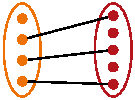
\includegraphics[width=0.85\linewidth]{\currentDir/1to1}}}%
%
\floatSep%
%
\subfloat[][%
A 1:N or 1-to-many relationship where participation on both ends is optional. %
An example would be the relation between supervising professors and students.%
\label{fig:relationshipCardinalities:1ton}%
]{\parbox{0.3\linewidth}{\centering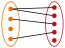
\includegraphics[width=0.85\linewidth]{\currentDir/1ton}}}%
%
\floatSep%
%
\subfloat[][%
A N:M or many-to-many relationship where participation on both ends is optional. %
An example would be the relation between students and course enrollments.%
\label{fig:relationshipCardinalities:ntom}%
]{\parbox{0.3\linewidth}{\centering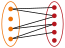
\includegraphics[width=0.85\linewidth]{\currentDir/ntom}}}%
%
\caption{Some simple examples for relationship cardinalities~\cite{SS2005EIDDDFDB:CDDICAMP,V1999C5DMS:CDUTERM}.}%
\label{fig:relationshipCardinalities}%
%
\end{figure}%
%
We already learned that attributes can have different cardinalities:
There can be single-valued or multi-valued attributes and either can be optional.
\Cref{fig:relationshipCardinalities} sketches a set of basic examples for relationship cardinalities.
Commonly, we distinguish one-to-one, one-to-many, and many-to-many relationships.
This is embodied by \citeauthor{C1976TERMTAUVOD}'s original \pgls{ERD} notation~\cite{C1976TERMTAUVOD}, where the relationship ends are simply annotated with 1, N, or M to express 1:1, 1:N, or M:N relationships.
In notation by \citeauthor{B1969DSD}~\cite{B1969DSD} from back in \citeyear{B1969DSD}, a relationship is represented by an arrow from one entity to another.
The entity to which the arrow points may occur N times, then one from which the arrow line originates once.

When creating an entity-relationship model, we often want a finer granularity.
We want to express whether relationships are optional or mandatory~(required) on either end of the relationship.
Therefore, usually, an end of relationships can be annotated with its modality~(is it optional or mandatory) and with its cardinality~(the number of participating entities)~\cite{R2024CDS:E}.
%
\begin{definition}[Relationship Modality]
The \emph{modality} of a relationship end defines whether participation is optional or mandatory. %
It can be viewed as the minimum number of participating entities.%
\end{definition}%
%
From a practical point of view, only the minimum participation numbers of 0 and~1 are practically relevant.
A modality of~0 means that relationship participation is optional.
In this case, one entity occurrence does not require a corresponding entity occurrence in a particular relationship.
A modality of~1 means that relationship participation is mandatory.
In this case, one entity occurrence requires a corresponding entity occurrence in a particular relationship.
This allows us to distinguish total and partial relationships~\cite{P2006CITRD:ERMI,V1999C5DMS:CDUTERM}.
If all entities of an entity set \emph{must} participate in at least one relationship, then this relationship end \emph{total}.
If only some entities participate in a relationship, then this relationship end is \emph{partial}.
%
\begin{definition}[Relationship Cardinality]
The maximum number of participating entities of a relationship end is called \emph{cardinality}.%
\end{definition}%
%
Practically, we usually only distinguish the cardinalities \emph{one} and \emph{many}, i.e., unlimited.%
In \pgls{UML}, cardinality is called multiplicity.

\begin{figure}%
\centering%
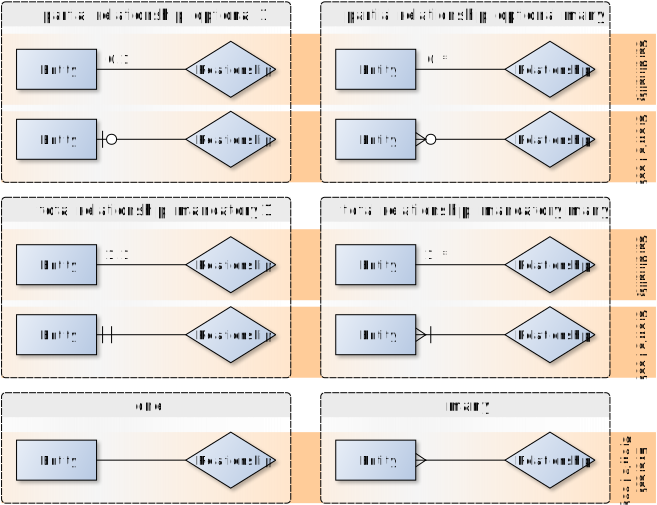
\includegraphics[scale=0.6]{\currentDir/erdCardinalities1}%
\caption{Two different ways to express possible modalities and cardinalities of relationship ends in \pglspl{ERD}.}%
\label{fig:erdCardinalities1}%
\end{figure}%

There are multiple conventions on how to express the relationship end modality and cardinality in an \pgls{ERD}.
\Cref{fig:erdCardinalities1} presents these two methods.
On one hand, there is the Crow's Foot notation~\cite{E1976BDSMEWACE,CM2000MDMAUDA,S2024D:CDMERDE}, where a graphical notation is used to expresses the cardinality and modality of a relationship end.
On the other hand, we can also directly write the permitted number of participants as labels on the ends the relationships~\cite{P2006CITRD:ERMI}.
Here, an integer range~\intRange{i}{j}, where $i$~is the minimum number of participating entities, $j$~is the maximum, and $*$~stands for unlimited, many, or~infinity.
The second method has the advantage of permitting much more diverse ranges of cardinalities.
The drawback is that it is slightly harder to draw, because we need to add labels to the relationship ends.
In \libreofficeBase, \pglspl{ERD} can be drawn that are directly linked to the underlying \db\ in the 1:1/1:N notation, but lowercase~n represent \inQuotes{many}.
\microsoftAccess\ offers a similar functionality, but the relationship ends are annotated with~1 or~$\infty$.
For the remainder of this text, we will stick to the Crow's Foot Notation to signify the relationship modalities and cardinalities~(while keeping \citeauthor{C1976TERMTAUVOD}'s notation for the symbols), simply because we can paint this more easily with \yEd\ without needing to add labels to relationship ends.

Notice that original Crow's Foot method by \citeauthor{E1976BDSMEWACE}~\cite{E1976BDSMEWACE}, also sketched in \cref{fig:erdCardinalities1}, which did not yet have the mandatory/optional symbolism.
This method can be used when the modality is not important during modeling, or when we want to leave it open and settle it during a later discussion.

Of course, there are many more possible notations to express the cardinality of relationships.
We could write $(i,j)$ instead of \intRange{i}{j} to express the possible numbers of participating entities~\cite{SS2005EIDDDFDB:CDDICAMP,G2011EW2ITDS:CMUTERM}.
Instead of using~$*$ as symbol for unlimited / many, some write M or N.
Different variations of the arrow-based notation are still in use as well.
An arrow touching the relationship diamond means \inQuotes{one} in~\cite{V1999C5DMS:CDUTERM}.
In~\cite{G2011EW2ITDS:CMUTERM}, the arrow needs to instead touch the entity rectangle and means either~$\geq0$ or~$\geq1$.
Nice overviews can be found in~\cite{B2025DS:AGTTERDE,S2012IITDM:AAAPGTERM}.
Which notation is used probably does not matter much, as long as all stakeholders agree upon and understand it.%
%
\begin{figure}%
\centering%
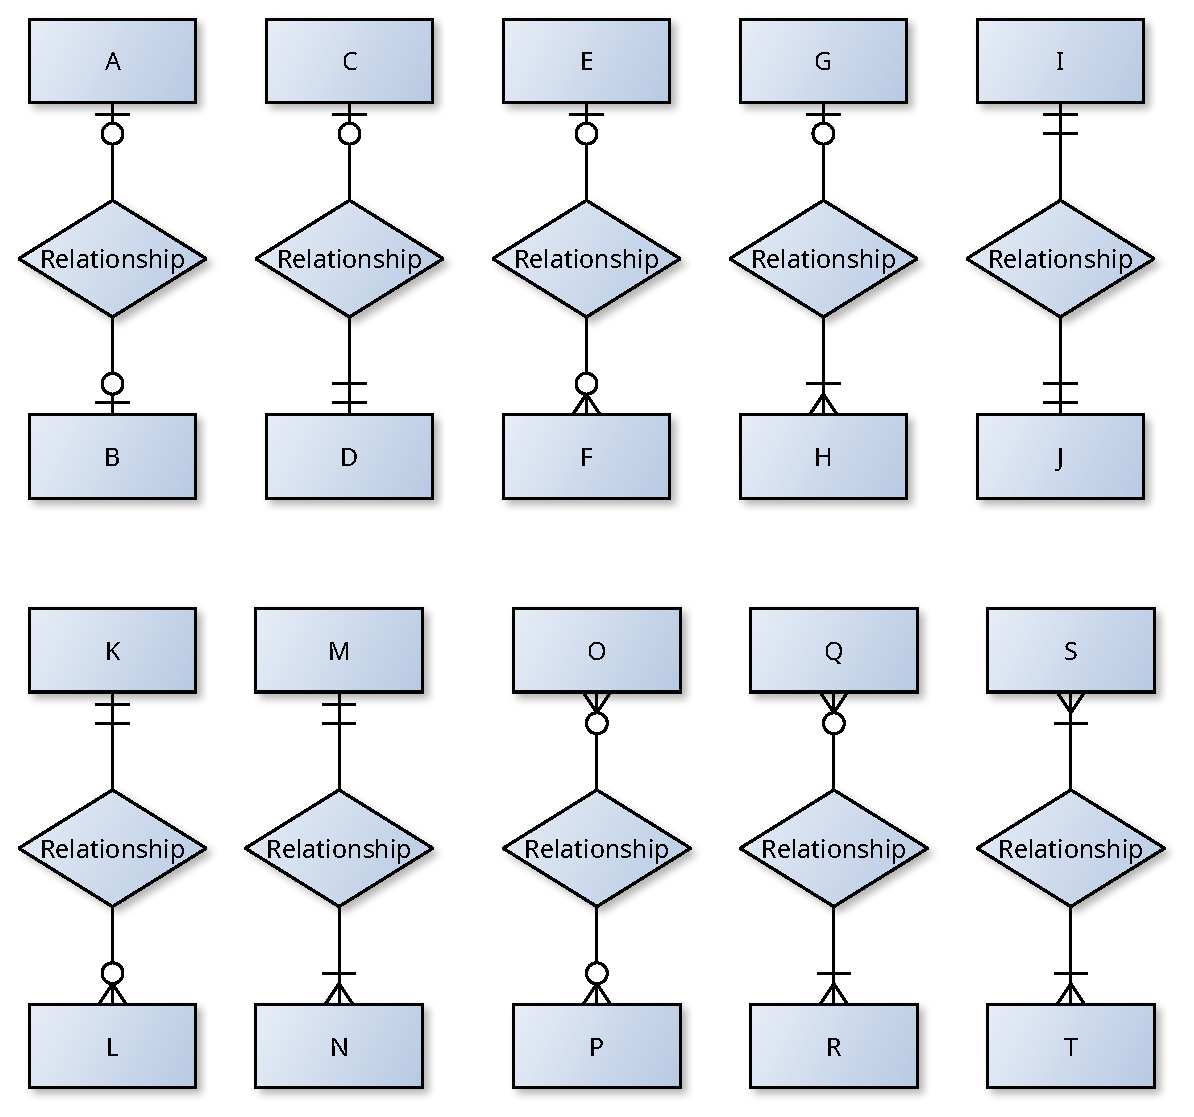
\includegraphics[scale=0.6]{\currentDir/erdCardinalities2}%
\caption{The ten possible combinations of cardinalities in Crow's Foot notation.}%
\label{fig:erdCardinalities2}%
\end{figure}%

As said, we will stick with the Crow's Foot notation, mainly because it is easy to use in \yEd.
Let's write down all the possible combinations of \inQuotes{relationship ends} in \cref{fig:erdCardinalities2} for this notation.
There are four possibilities to annotate the end of a relation:%
\begin{itemize}%
\item Optional~1:~\crowsFootOptionalOne, equivalent to~\intRange{0}{1},%
\item Mandatory~1:~\crowsFootMandatoryOne, equivalent to~\intRange{1}{1},%
\item Optional~Many:~\crowsFootOptionalMany, equivalent to~\intRange{0}{*}, \intRange{0}{\textnormal{N}}, and~\intRange{0}{\infty}, and%
\item Mandatory~Many:~\crowsFootMandatoryMany, equivalent to~\intRange{1}{*}, \intRange{1}{\textnormal{N}}, and~\intRange{1}{\infty}.%
\end{itemize}%
%
Since each relationship as two ends, this gives us $4+3+2+1=10$ different combinations.
It is important to understand how to interpret the cardinalities and modalities of the relationship ends, because this can easily be mistaken:
The participation of an entity depends on the \emph{other} end.
Let's take \crowsFoot{K}{M1}{L}{OM} as example.
First, place your finger on the~K as say \inQuotes{Each~K has\dots}.
Now move your finger towards the~L and read the relationship end there says:~\inQuotes{{\dots}one to many~L.}~\cite{R2016HDIRENCFTCTNL}.
Then place your finger on the~L an say \inQuotes{Each~L has\dots}.
Move the finger to the~K and read the relationship end touching the~K.
This means that~\inQuotes{{\dots}exactly one~K.}
Notice that the \crowsFootMandatoryOne\ touching~K does \emph{not} mean that \inQuotes{Every K must be related to some~L.}
To be on the safe side, let's write down the meaning of each of them based on \cref{fig:erdCardinalities2}.%
%
\begin{itemize}%
%
\item \crowsFoot{A}{O1}{B:}{O1} Each~A may be linked to zero or one~B. Each~B may be linked to zero or one~A.~\cite{BS2023G:CFNIERD}\\%
\emph{Example:}~When issuing an order for goods online, a customer may enter a discount code.
Each discount code must be used at most once.
At most one discount code can be used for an order.~\cite{BS2023G:CFNIERD}\\%
\emph{Example:}~One person maybe married to another person.~\cite{R2024CDS:E}%
%
\item \crowsFoot{C}{O1}{D:}{M1} Each~C must be linked to exactly one~D. Each~D may be linked to zero or one~C.~\cite{T2025CDBMS:ERM}\\%
\emph{Example:}~Each office in an office building may host zero or one salespersons.
Each salesperson must have one office.~\cite{T2025CDBMS:ERM}\\%
\emph{Example:}~A professor may be the dean of school or not be a dean.
A school must have exactly one dean.~\cite{R2024CDS:E}%
%
\item \crowsFoot{E}{O1}{F:}{OM} Each~E may be linked to zero, one, or many~F. Each~F may be linked to at most one~E.~\cite{MA2006MAC:DMERDED}\\%
\emph{Example:}~Assume that for bank accounts, two addresses may be associated:
A home address is required~(not relevant for this example).
Additionally, a bank account may be linked to zero or one postal address.
Each address may be the postal address of zero, one, or many bank accounts.~\cite{MA2006MAC:DMERDED}%
%
\item \crowsFoot{G}{O1}{H:}{MM} Each~G is related at least one, but maybe many~H. Each~H may or may not be linked to a~G, but never to more than one~G.%
%
\item \crowsFoot{I}{M1}{J:}{M1} Each~I must be associated with exactly one~J. Each~J must be associated with exactly one~I.\\%
\emph{Example:}~In a company, one salesperson must be the backup for each~(other) salesperson.
Each salesperson is the backup of one salesperson.~\cite{T2025CDBMS:ERM}%
%
\item \crowsFoot{K}{M1}{L:}{OM} Each~K may be linked to zero or many~L. Each~L must be linked to exactly one~K.~\cite{MA2006MAC:DMERDED,BS2023G:CFNIERD}\\%
\emph{Example:}~A customer may issue zero or arbitrarily many orders for products.
However, each order must be linked to exactly one customer.~\cite{BS2023G:CFNIERD}\\%
\emph{Example:}~A bank account may take part in zero, one, or many bank transfers as source account.
However, each bank transfer must have exactly one source bank account.~\cite{MA2006MAC:DMERDED}\\%
\emph{Example:}~Each customer is handled by exactly one salesperson.
A salesperson may not have any customers, one customer, or many customers.~\cite{T2025CDBMS:ERM}%
%
\item \crowsFoot{M}{M1}{N:}{MM} Each~M is related to at least one and possibly multiple~N. Each~N is related to exactly one~M.~\cite{BS2023G:EDFAHMSCFN}\\%
\emph{Example:}~A patient can make several appointments~(to visit doctors).
Each appointment is linked to exactly one patient.~\cite{BS2023G:EDFAHMSCFN}\\%
\emph{Example:}~A school of a university must consist of at least one, but possibly many departments.
Each department must belong to exactly one school.~\cite{R2024CDS:E}%
%
\item \crowsFoot{O}{OM}{P:}{OM} Each~O may be related to zero, one, or multiple~P. Each~P may be related to zero, one, or multiple~Q.\\%
\emph{Example:}~A pizza shop sells pizza to customers.
A pizza may be ordered by zero, one, or many customers.
A customer may not order pizza~(maybe the want to eat something else), or order one pizza, or order multiple pizzas.~\cite{FCC2016D:CFNRSAHTRD}%
%
\item \crowsFoot{Q}{OM}{R:}{MM} Each~Q must be linked to at least one~R, i.e, one or many~R. Each~R may be related to zero or many~Q.~\cite{BS2023G:CFNIERD}\\%
\emph{Example:}~When placing an order for products online, the order must be for at least one product.
Each product may be referenced by zero, one, or many orders.~\cite{BS2023G:CFNIERD}%
%
\item \crowsFoot{S}{MM}{T:}{MM} Each~S is linked to at least one~T. Each~T is linked to at least one~S.~\cite{T2025CDBMS:ERM}\\%
\emph{Example:}~Each salesperson sells at least one product but may also sell more than one product.
Each product by be sold by one salesperson, but also by many salespeople.~\cite{T2025CDBMS:ERM}
%
\end{itemize}%
%
\FloatBarrier%
%
\begin{figure}%
\centering%
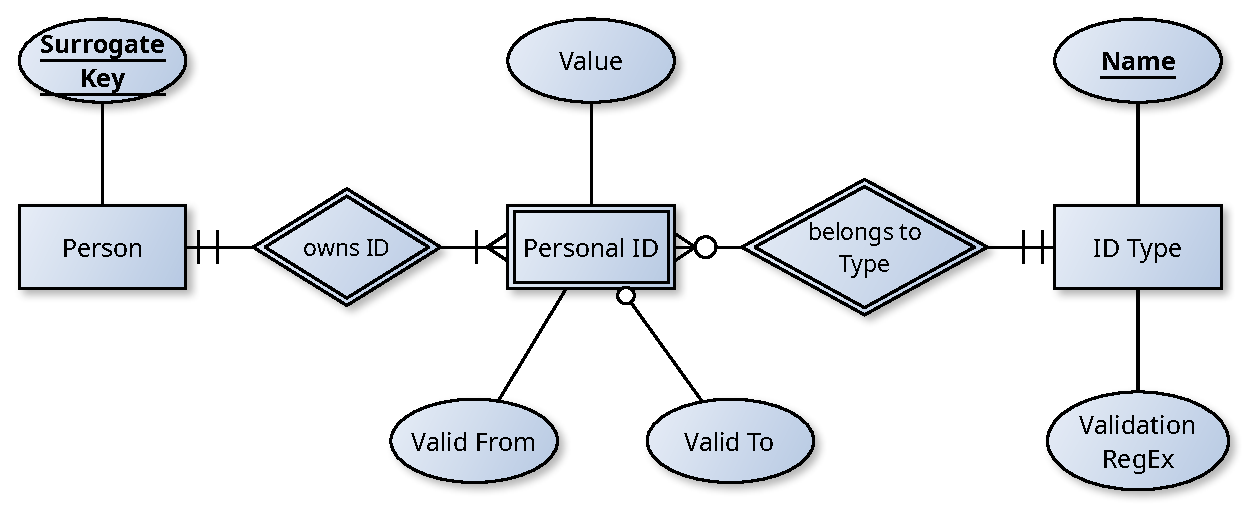
\includegraphics[scale=0.6]{\currentDir/erdPerson4}%
\caption{The \pgls{ERD} for \emph{Person} from \cref{fig:erdPerson3}, but annotated with relationship cardinalities.}%
\label{fig:erdPerson4}%
\end{figure}%

So let us now annotate the cardinalities to the relationships of the \emph{Person} entity type from \cref{fig:erdPerson3}.
This leads to the new \pgls{ERD} in \cref{fig:erdPerson4}.
We had the idea to have multiple different \emph{ID~Types}.
Each actual \emph{Personal~ID} must belong to exactly one~\emph{ID~Type}.
There may be an arbitrary number of \emph{Personal~ID}s for each \emph{ID~Type} in our system, maybe none at all, maybe one, maybe many.
Hence, the relationship is \crowsFoot{\emph{Personal~ID}}{OM}{\emph{ID~Type}}{M1}.

Each \emph{Personal~ID} belongs to exactly one \emph{Person}.
At the same time, there must be at least one \emph{Personal~ID} for every \emph{Person} record in our \db.
We cannot have any person in our system whose identify has not been confirmed in at least one official way.
Thus, the relationship will be \crowsFoot{\emph{Person}}{M1}{\emph{Personal~ID}}{MM}.

\begin{figure}%
\centering%
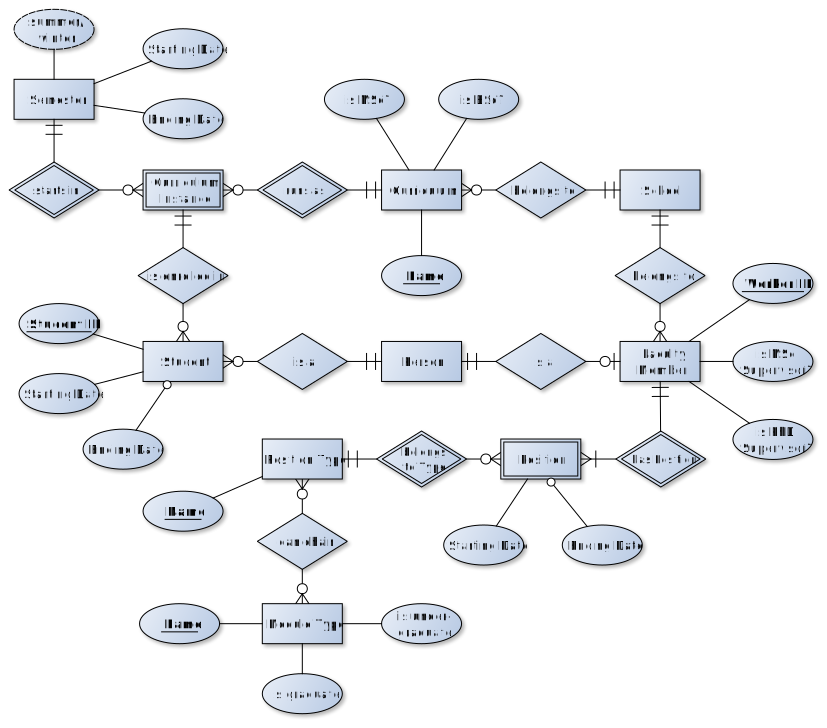
\includegraphics[width=0.99\linewidth]{\currentDir/erdPersonStudentFaculty2}%
\caption{A significant extension of the \cref{fig:erdPersonStudentFaculty1} \pgls{ERD} describing the relationship between students, professors, and persons. %
The new diagram also introduces curricula, schools, and positions.}%
\label{fig:erdPersonStudentFaculty2}%
\end{figure}%

In \cref{fig:erdPersonStudentFaculty2}, we now expand our \pgls{ERD} regarding the two different types of persons, namely students and professors.
We know that each student record must be associated with exactly one person record, because each student is a person and only one person.
Then again, a person record may be associated with zero student roles~(if they are not a student) or one student role~(e.g., they enrolled as compute science Bachelor student).
However, a person may also have \emph{multiple} student roles.
Maybe they enrolled as computer science Bachelor student, completed this curriculum and then graduated.
Then they enrolled in the Master's program for computer science.
In this case, they receive a new student~ID.
Each student role has a starting date and an end date.

Every student must be enrolled in exactly one curriculum instance.
There may be zero, one, or many students enrolled in a curriculum instance.
What is a curriculum instance?
Well, we said that a student is maybe enrolled in the Bachelor program for computer science.
When they do so, they enroll in a particular semester of the program, say, the Bachelor program computer science starting in the Winter semester of~2024.
From the perspective of entity relationship modeling, we could say:
A curriculum may be executed by the university zero~(unlikely), one, or many times as curriculum instance.
Each curriculum instance is associated with exactly one curriculum.
Also, it is associated with exactly one semester.
Since curricula instances do not have any other identifying characteristics and cannot exist by themselves, they are weak entities.
They only come to life through their relationship with the curriculum they belong to and the semester in which they are launched.

We decided to model a semester as independent entity, because this allows us to tag attributes to it.
For example, a semester can have a start date and end date, it may even have dates for the exam period.
Since we give the start and end date, we could derive attributes such as whether a semester is a summer or a winter semester.
Of course, in each semester, our university may launch zero, one, or many instances of curricula.

A curriculum has a unique name, serving as its primary key.
Curricula also have further attributes, e.g., whether they are undergraduate or graduate programs.
Each curriculum belongs to exactly one school of our university.
Each school may have zero, one, or many curricula.

This model describes the situation of the students reasonably well.
By tracing the relationships, we know which curriculum a student attends.
We did not model this, but you can assume that, to each curriculum, we can relate the modules that it contains and in which semester of the curriculum they need to take place.
Hence, we would know when which student should attend which module.
We also know to which school a student belongs to.
Based on this, the set of professors who could be their supervisor can be constructed.

Let us now model a bit of the situation of faculty members.
A person can be at most one faculty member.
Each faculty member is exactly one person and has a unique worker's~ID.
This is a bit different from the situation of students:
A student gets a new student~ID every time they enroll into a curriculum.
The most common case is that a student will only study one curriculum in our university.
A faculty member, however, will always retain the same worker's~ID.
A faculty member may be promoted or change their position, but the worker's~ID will never change.

There are different types of positions in a university.
For example, lecturer, assistant professor, associate professor, full professor, and even different levels of full professorship.
Each such position type has a unique name and determines which kind of things a faculty member can do.
For example, there are different types of modules, such as undergraduate modules, graduate modules, professional base classes, professional special classes, etc.
A person at a given position type may chair modules belonging to an arbitrary number of module types.
Each module type may be chaired by faculty members belonging to an arbitrary number of position types.

Either way, we introduce the weak entity position that we use to link faculty members to position types.
Every instance of this weak entity belongs to exactly one faculty member and to exactly one position type.
Each faculty member does have at least one position.
Usually they have only one position at a time~(which is why each position has a starting date and an optional end date).
Faculty members may have multiple different positions over time, for example, they may start as lecturer in 2022, then be promoted to associate professor in 2025.
For each position type, there may be arbitrarily many corresponding position records.

Interestingly, whether a faculty member can supervise certain types of students is not necessarily only determined by the position type.
These abilities are instead attributes of the faculty member.
They may require certain positions, such as full professor for graduate students.
But there may also be other factors, such as recent publications, fulfillment of teaching duties, etc.

Finally, we also model that each faculty member belongs to exactly one school.
An each school can have an arbitrary number of faculty members.

When we look at the new \cref{fig:erdPersonStudentFaculty2}, we find that it is truly beautiful.
We can also see that many things are still missing.
For example, we did not yet model the relationship between students and classes, classes and modules, modules and curricula, classes and rooms, the list of available rooms and their features, exams, exam results, graduation requirements, and so on.
Still, we have managed to drag a good piece of reality into our model.%
%
\FloatBarrier%
\endhsection%
%
